\section{Utilizzo applicazione}
	\subsection{Aggiunta dei dati di addestramento}
	Per aggiungere i dati di addestramento, cliccare sul pulsante "Seleziona un file csv".
	\begin{figure}[H] 	
		\begin{center}
			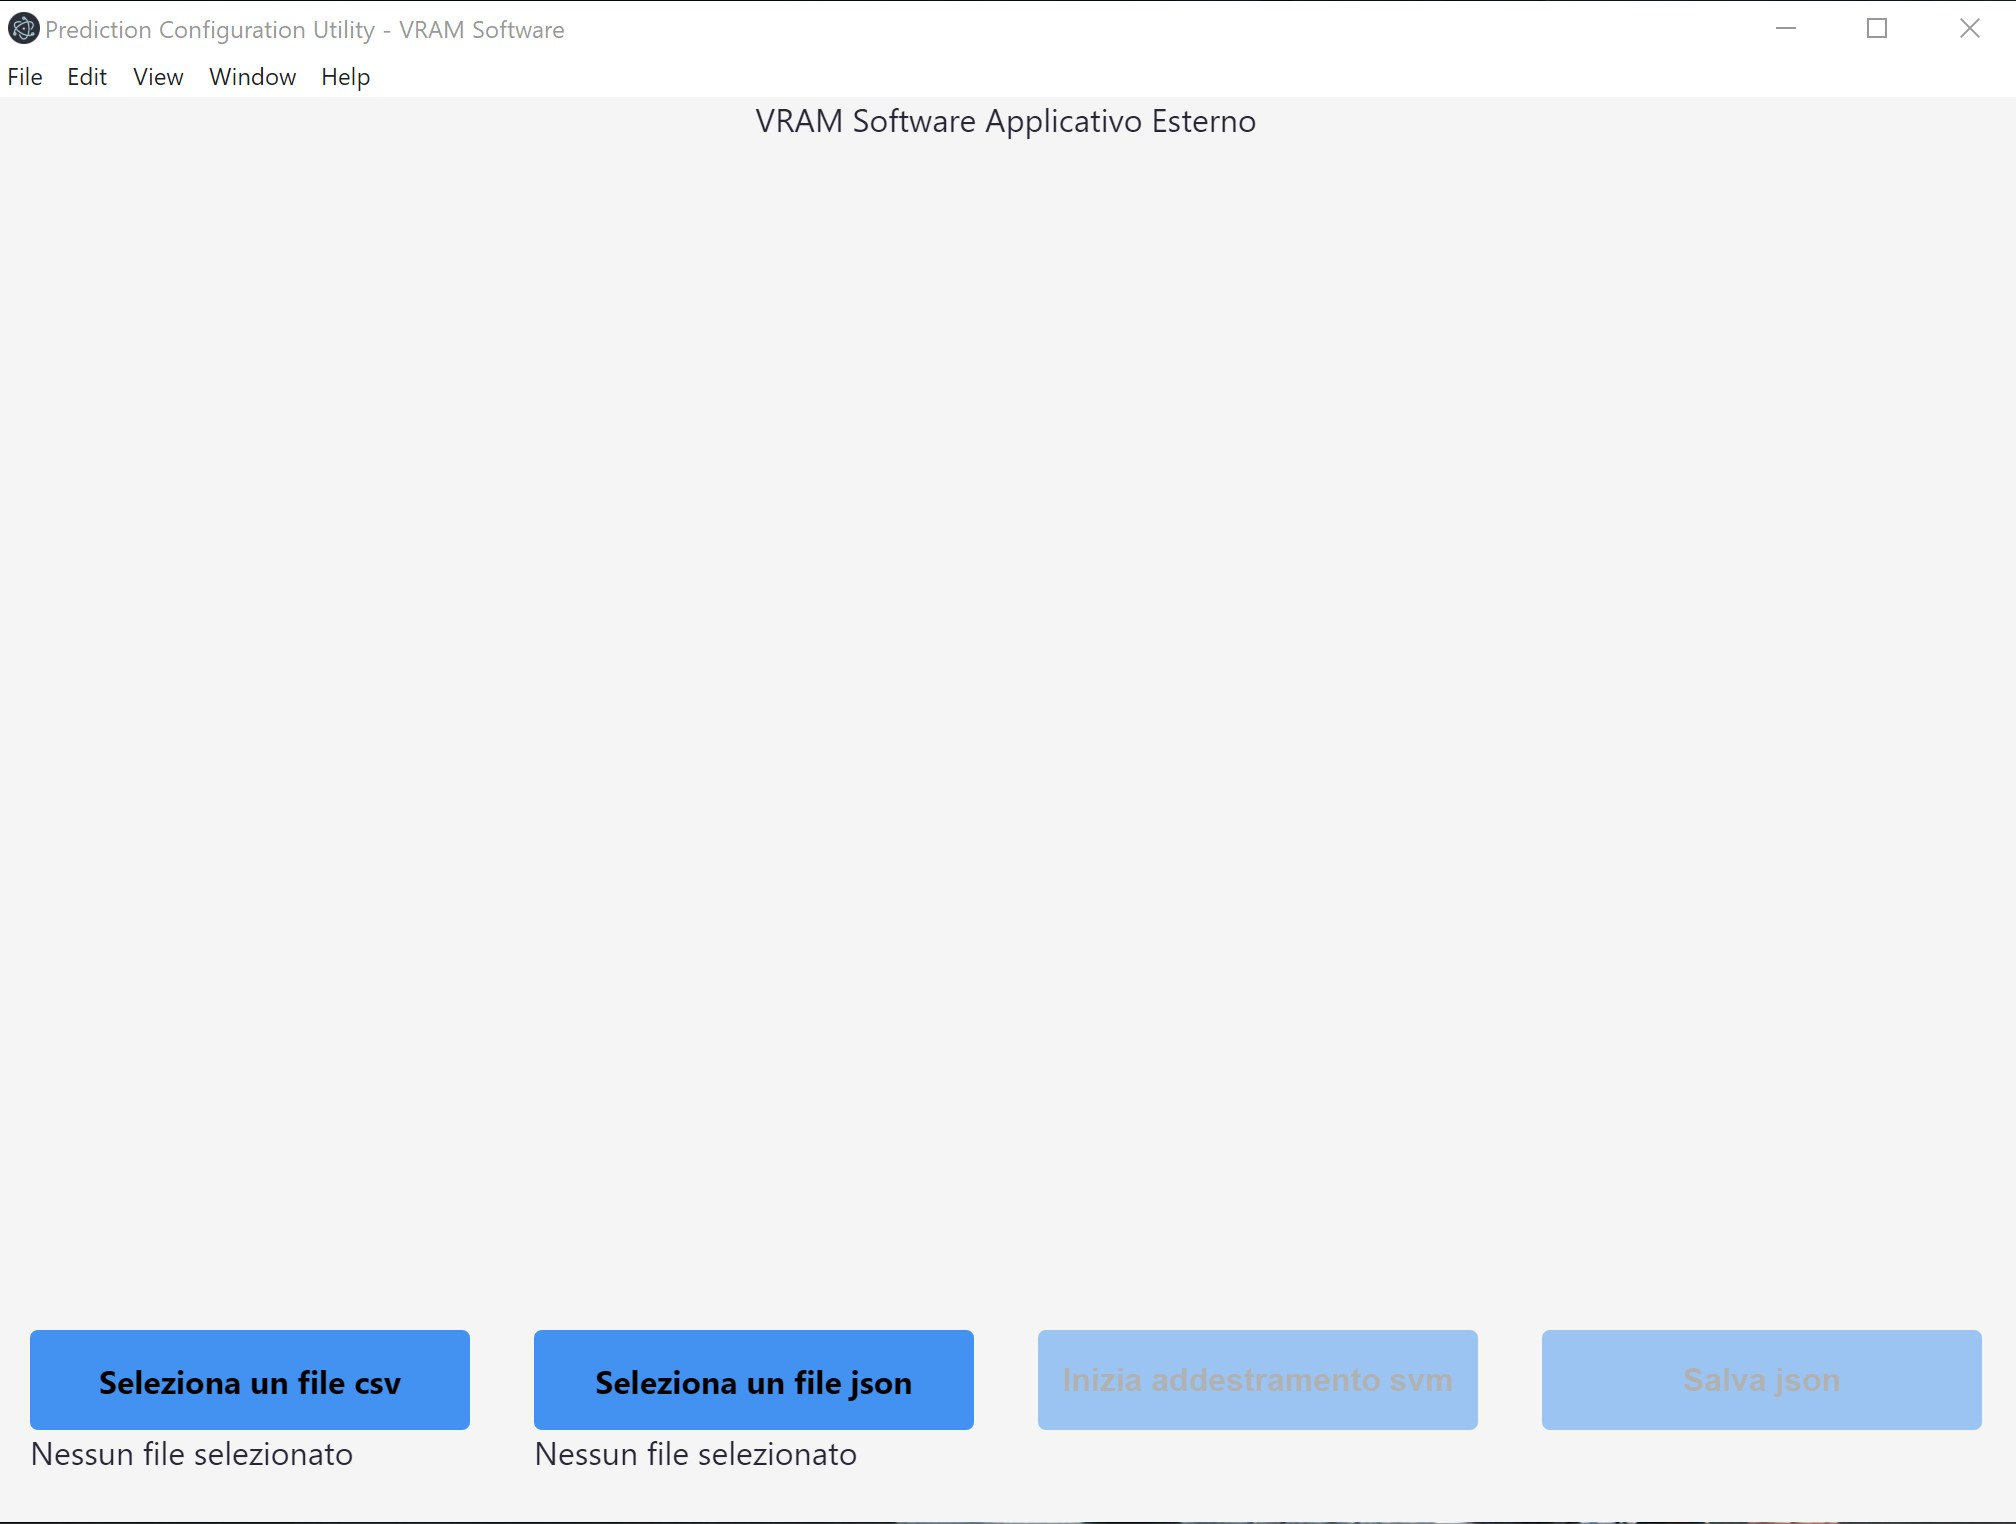
\includegraphics[width=\linewidth]{img/1.jpg}
		\end{center}
		\caption{Seleziona file csv}	
	\end{figure}
	Si aprirà il file manager di sistema e sarà possibile importare il file desiderato. Una volta selezionato apparirà un pop-up dove sarà possibile scegliere l'algoritmo di predizione che ci desidera addestrare per quei dati, selezionare l'ordine dei predittori e selezionare l'ordine dei predetti.
	\begin{figure}[H] 	
		\begin{center}
			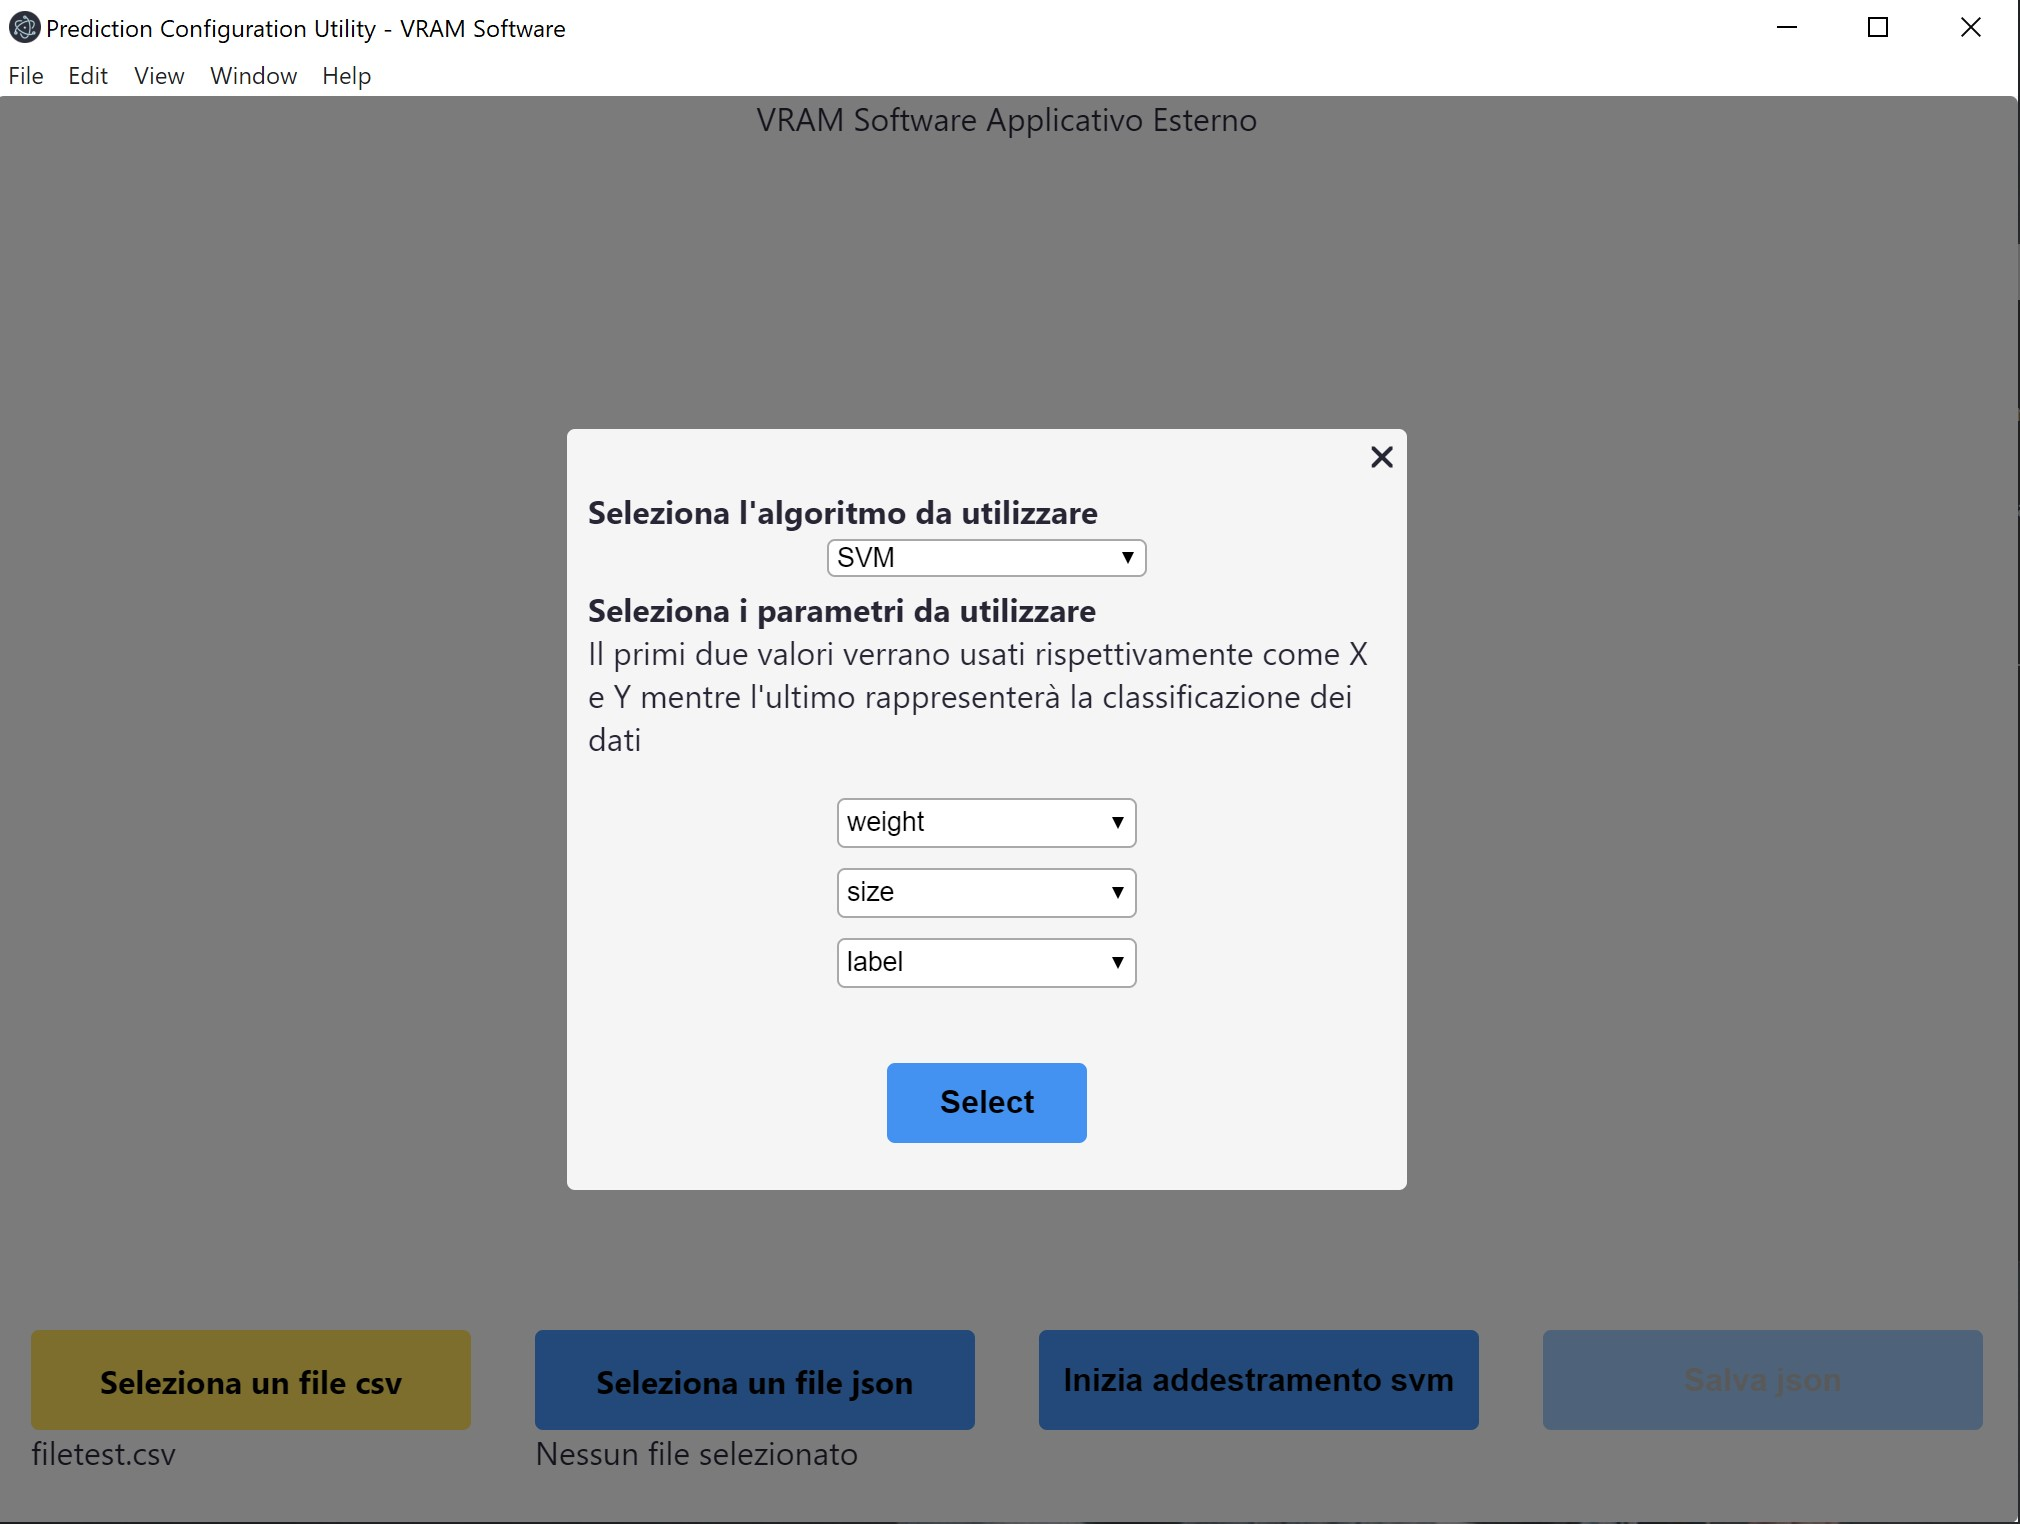
\includegraphics[width=\linewidth]{img/2.jpg}
		\end{center}
		\caption{Selezione dell'algoritmo e dei parametri di predizione}	
	\end{figure}
	Una volta selezionati apparirà un grafico in base all'ordine scelto.
	\subsection{Aggiunta di un file di configurazione}
	Per aggiungere un file di configurazione precedentemente già creato, cliccare sul pulsante "Seleziona un file json".
	Si aprirà il file manager di sistema e sarà possibile importare il file desiderato. Una volta selezionato verranno automaticamente aggiornate le note dell'addestramento.
	%\begin{figure}[H] 	
	%	\begin{center}
	%		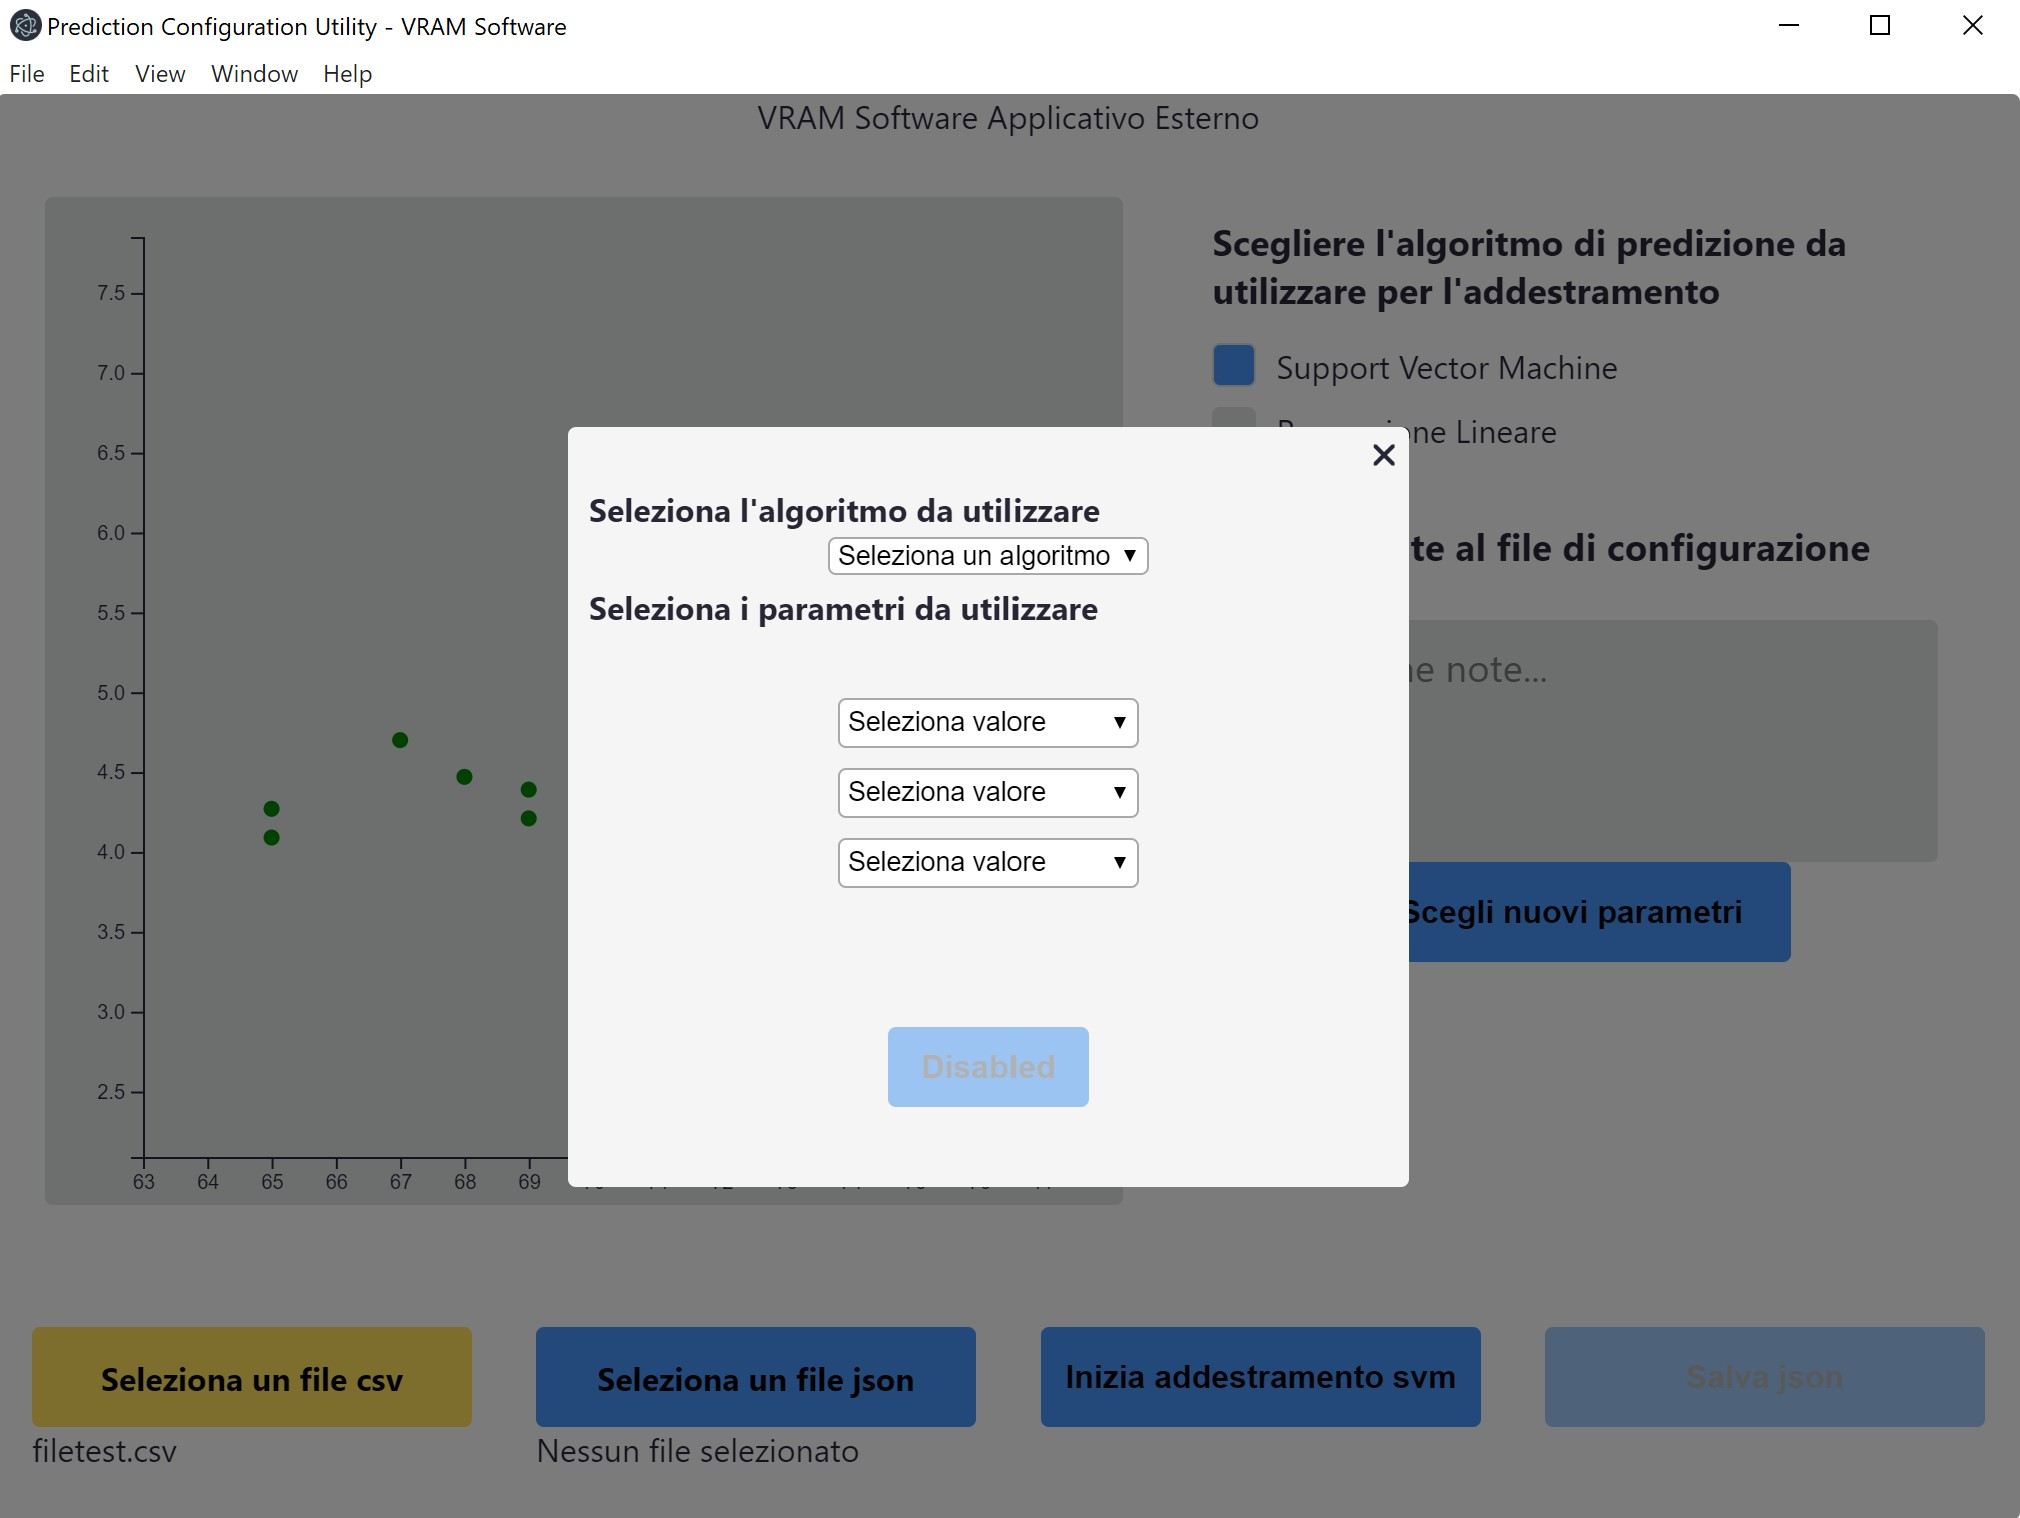
\includegraphics[width=\linewidth]{img/3.jpg}
	%	\end{center}
	%	\caption{Seleziona file Json}	
	%\end{figure}
	\subsection{Avvio dell'addestramento}
	Una volta aggiunti i dati di addestramento sarà possibile cliccare sul pulsante "Avvio addestramento". Al termine dell'addestramento verrà visualizzato il messaggio "Addestramento avvenuto" e, se le dimensioni dei dati lo consentono, il risultato sarà visualizzabile nel grafico.
	\begin{figure}[H] 	
		\begin{center}
			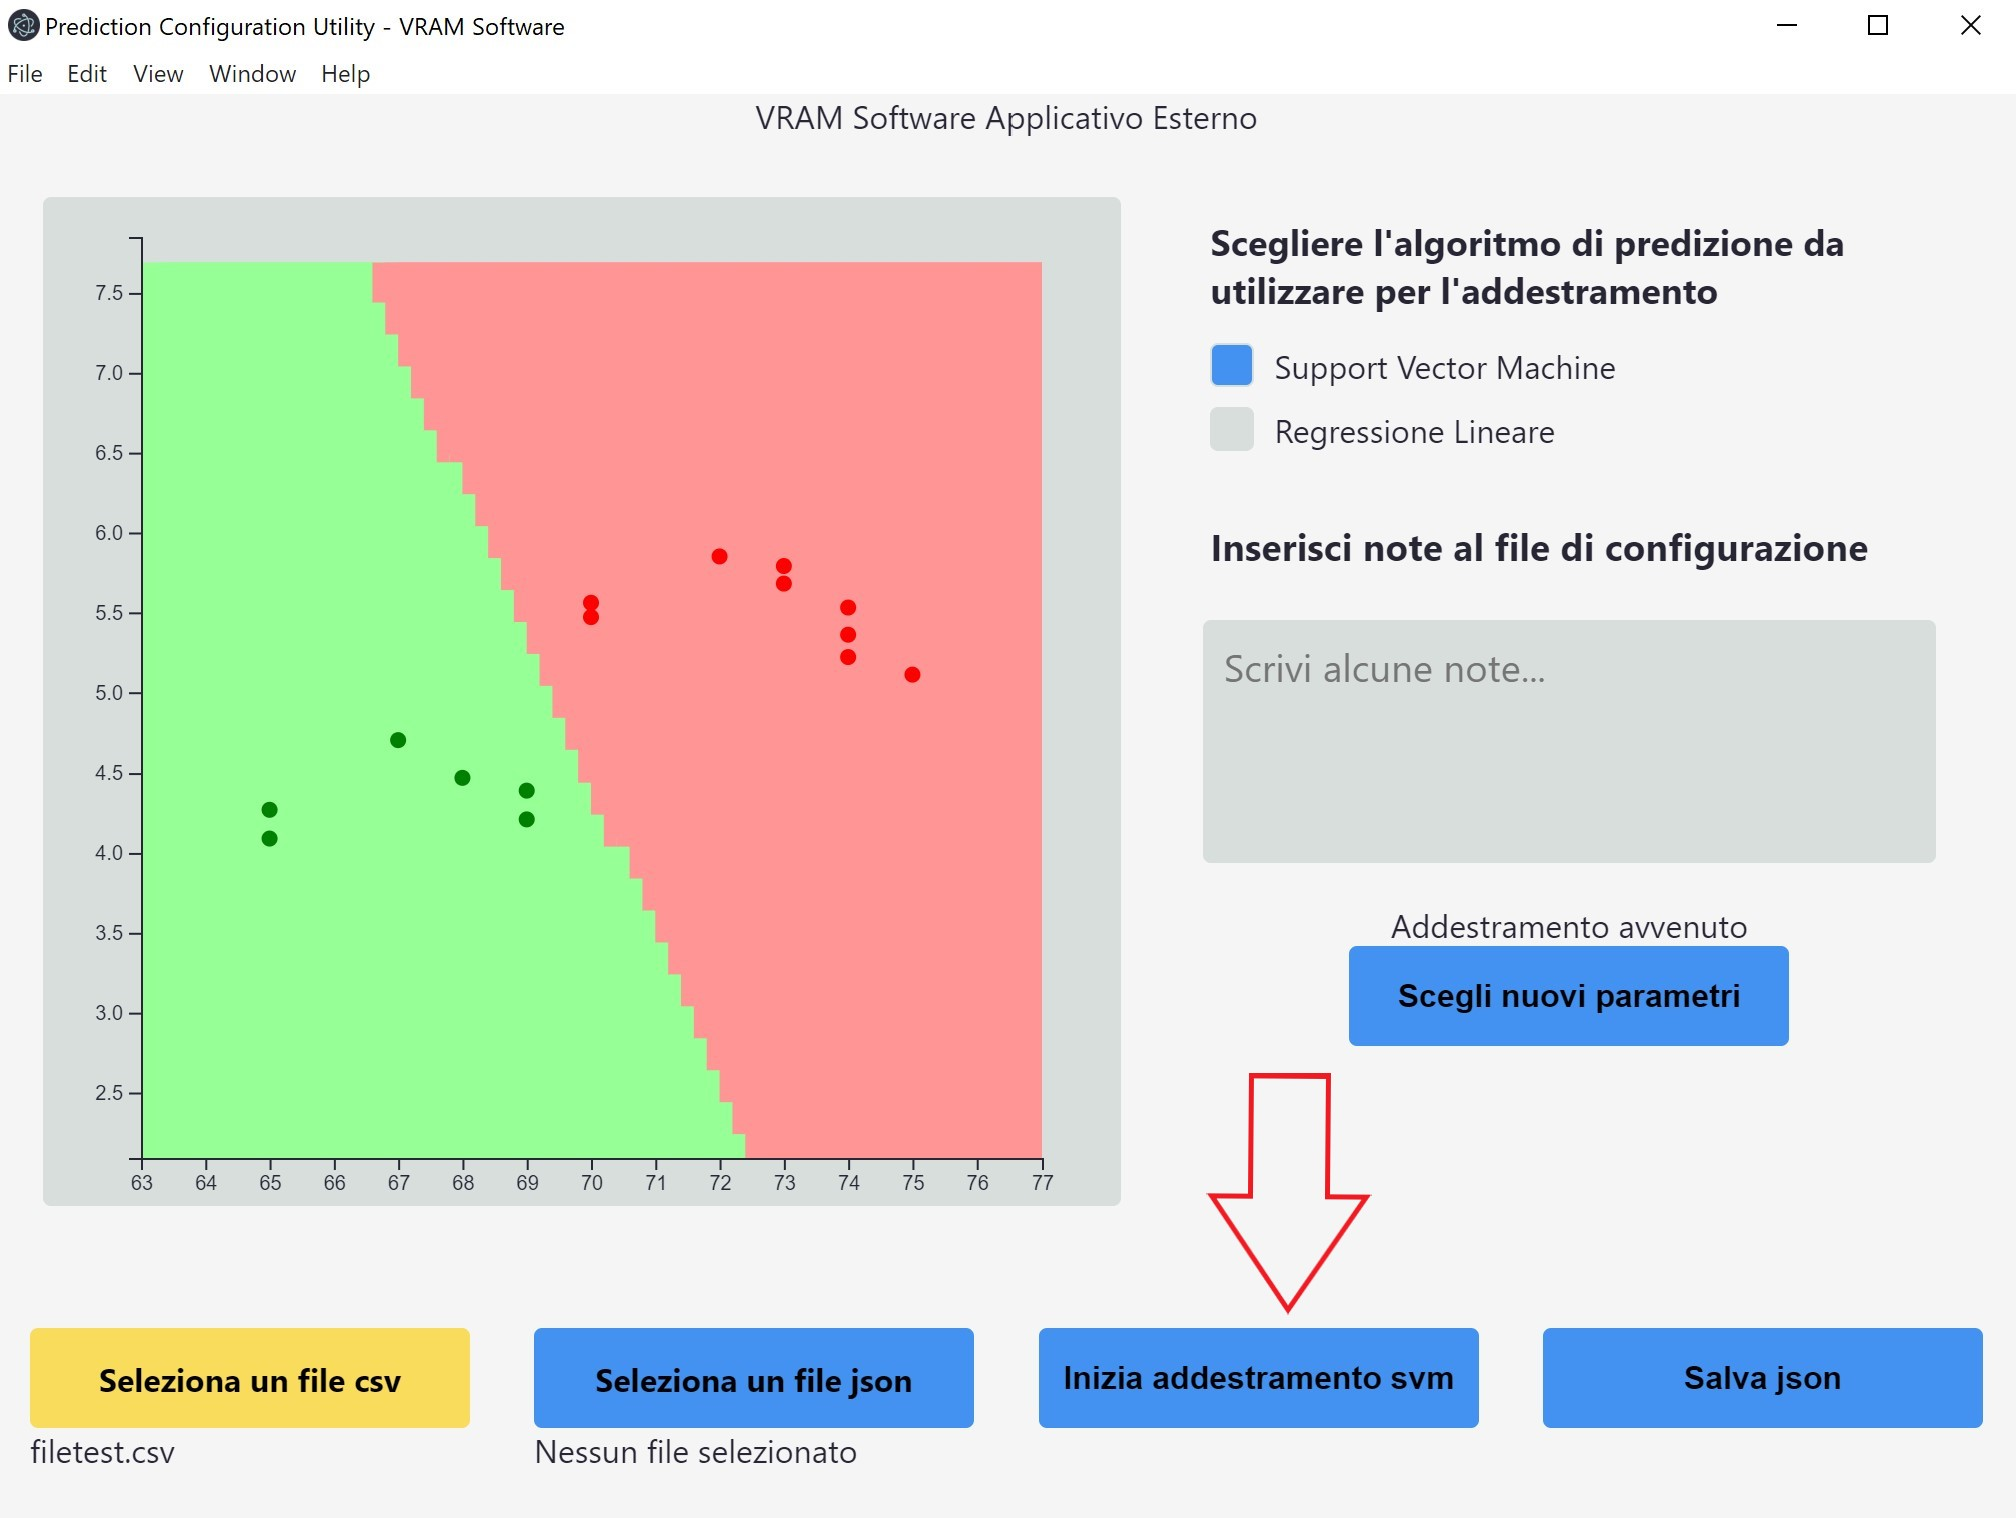
\includegraphics[width=\linewidth]{img/4-3.jpg}
		\end{center}
		\caption{Avvio dell'addestramento}	
	\end{figure}
	\subsection{Cambio dei parametri}
	Cliccando sul pulsante "Cambia parametri" apparirà un pop-up dove sarà possibile cambiare l'ordine dei predittori e dei predetti come avviene nell'inserimento del file.
	\begin{figure}[H] 	
		\begin{center}
			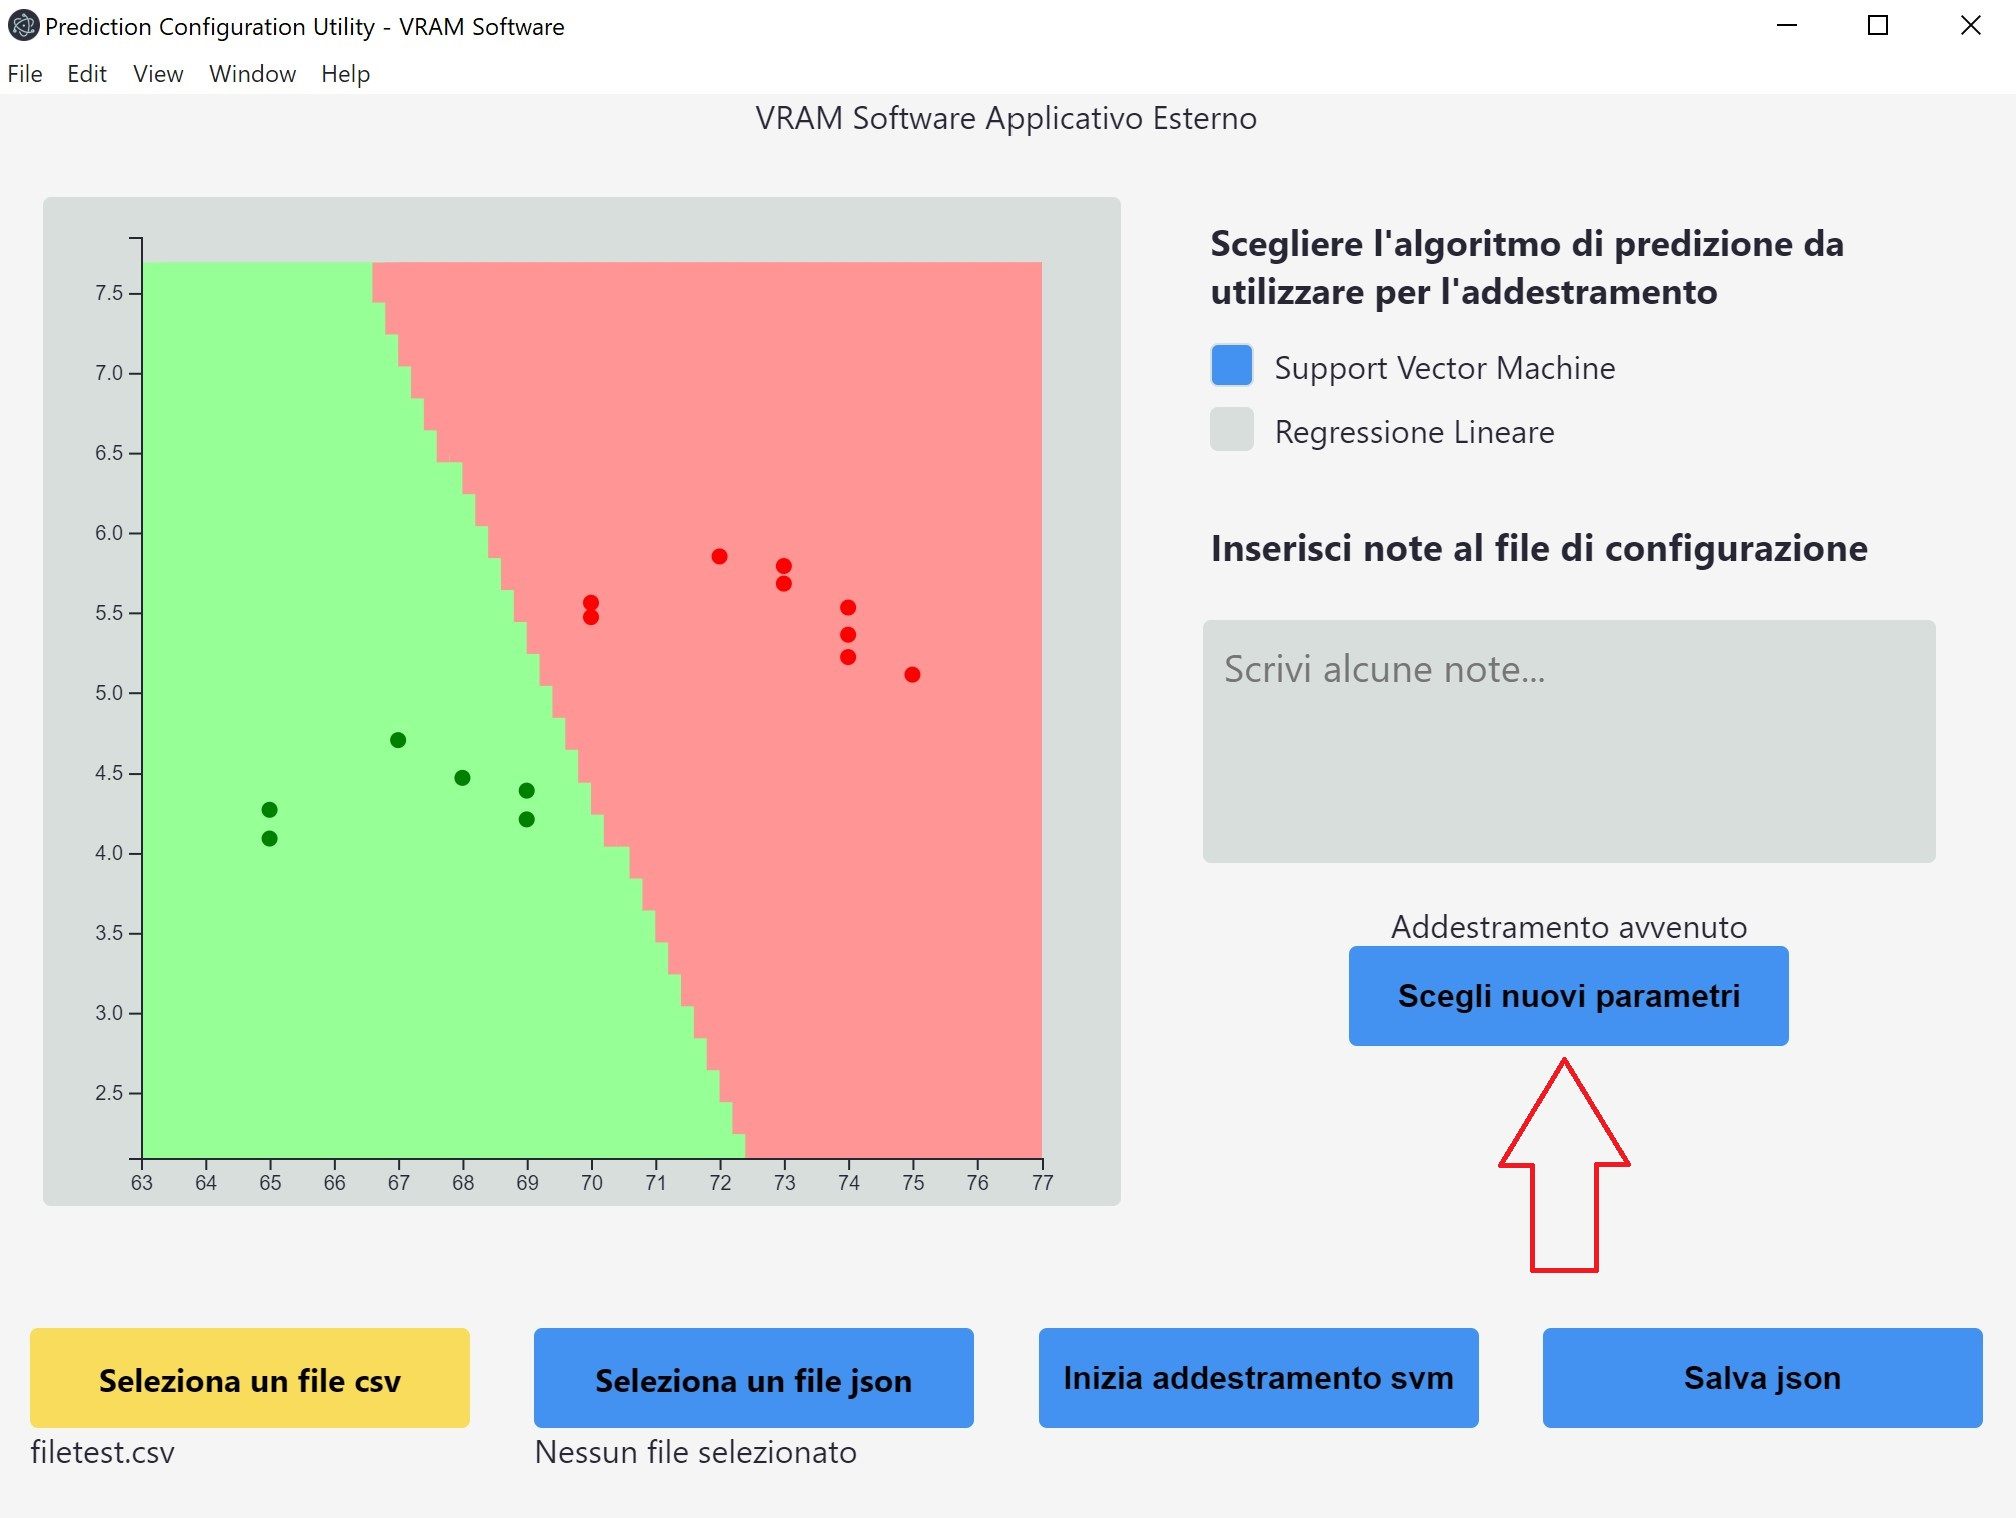
\includegraphics[width=\linewidth]{img/4-1.jpg}
		\end{center}
		\caption{Cambio dei parametri di addestramento}	
	\end{figure}
	\subsection{Salvataggio dei risultati}
	Cliccando sul pulsante "Salva json" apparirà un pop-up in cui si potrà inserire il nome del file e salvarlo sulla cartella "output". Questo file conterrà tutte le informazioni dell'addestramento necessarie per eseguire la predizione e le eventuali note scritte nel box dell'applicazione.
	\begin{figure}[H] 	
		\begin{center}
			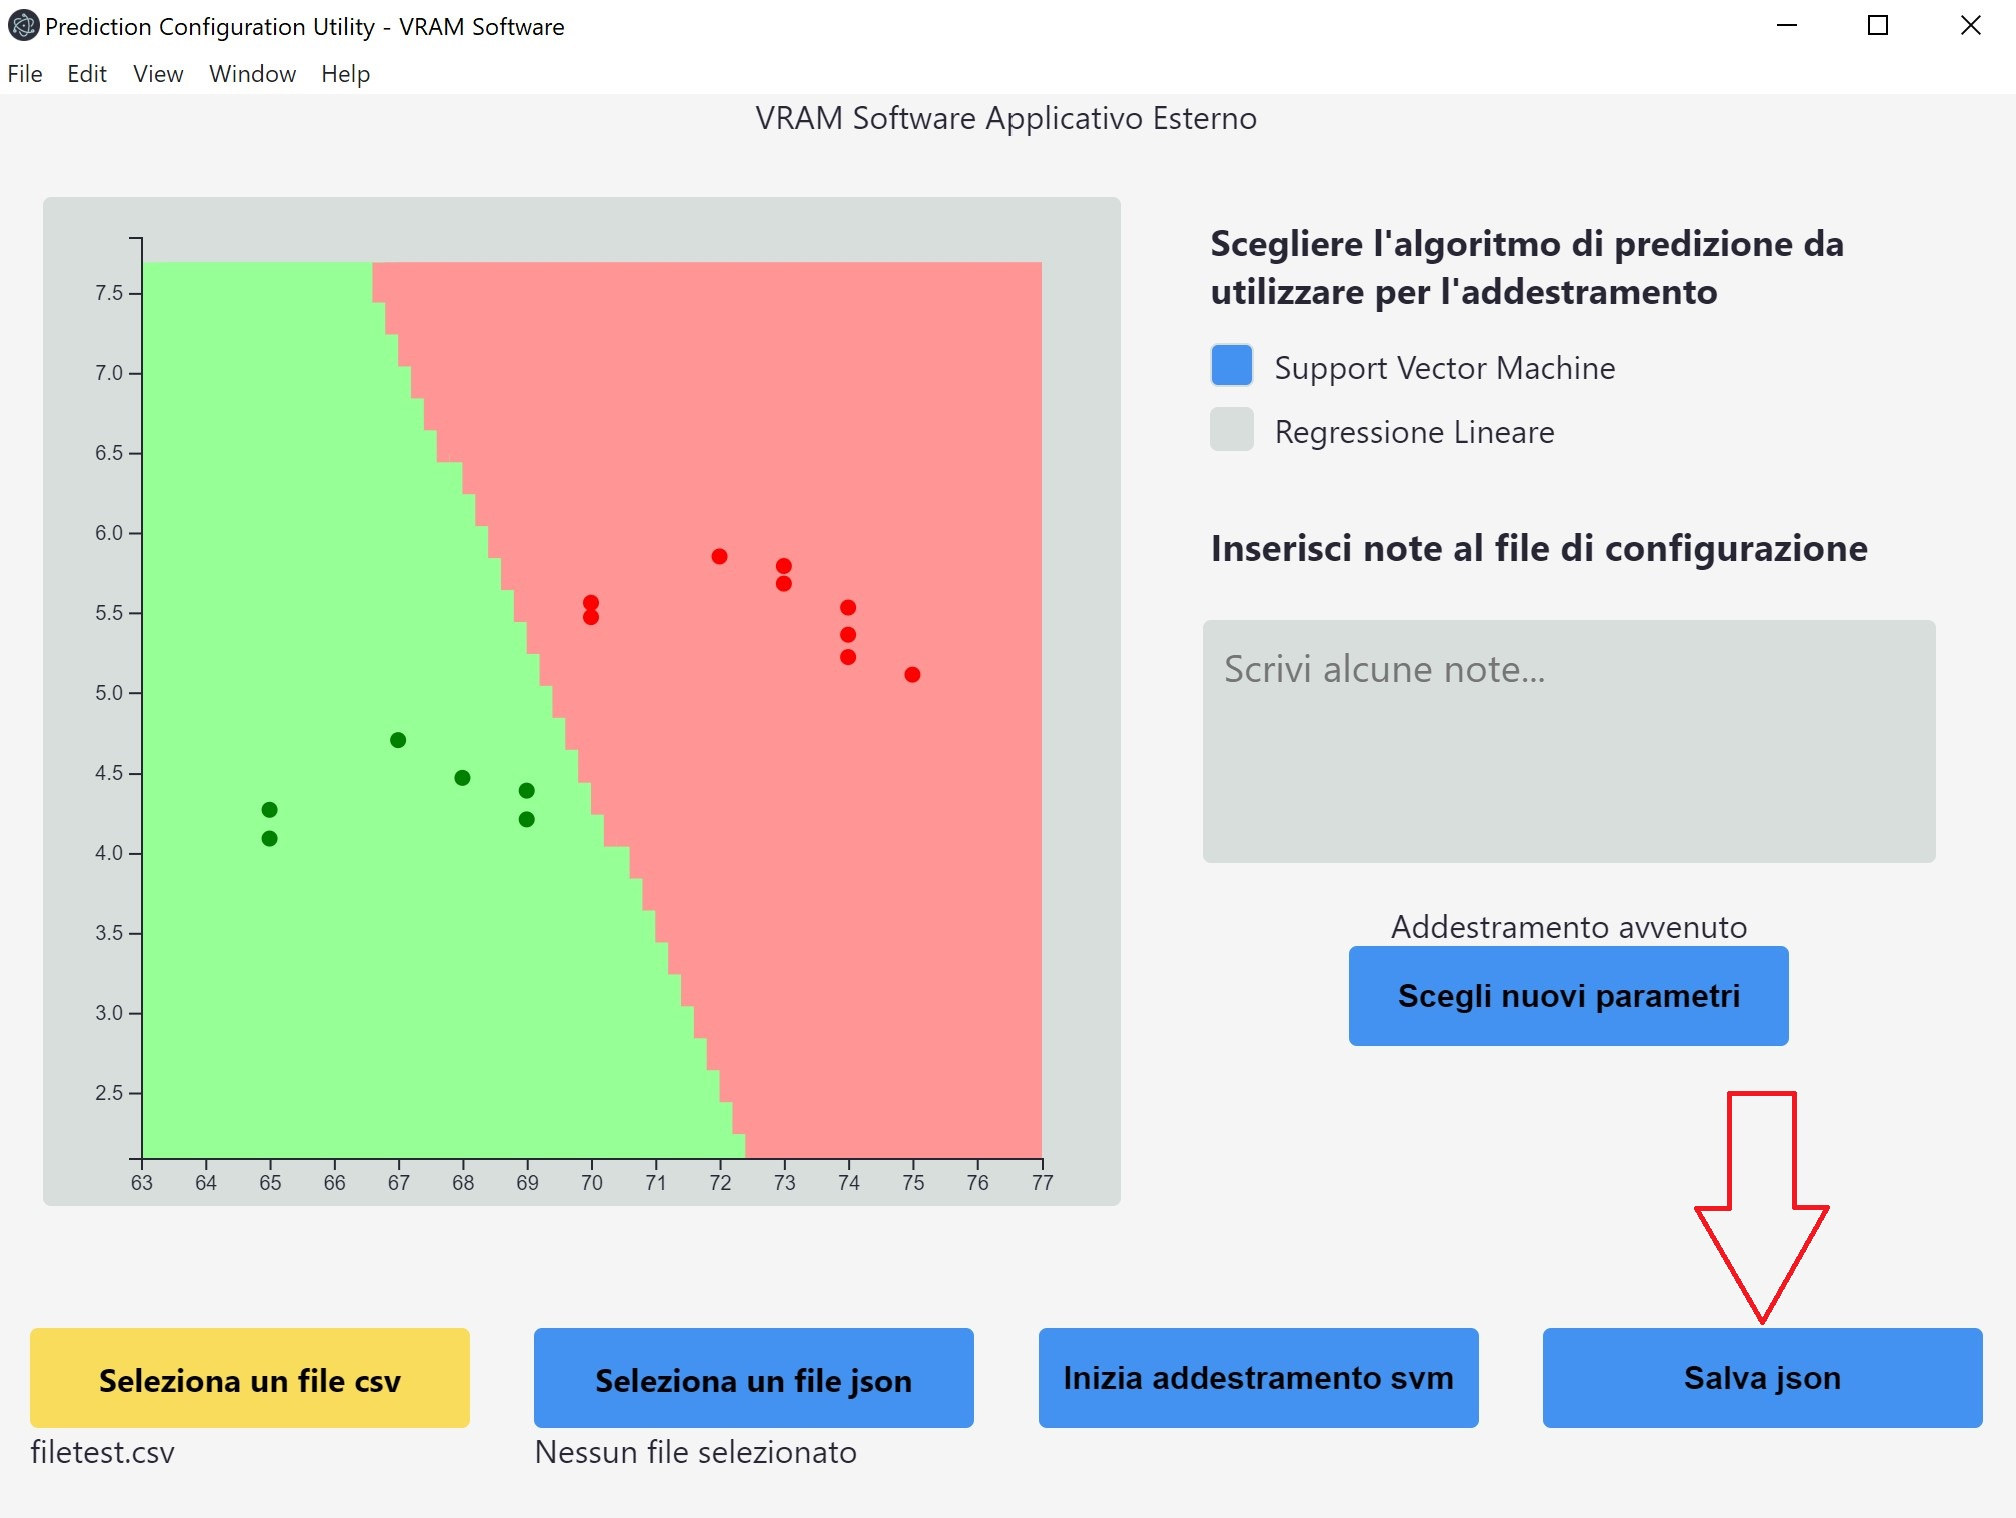
\includegraphics[width=\linewidth]{img/4-2.jpg}
		\end{center}
		\caption{Salva file Json}	
	\end{figure}
	
